\section{Personnalisation du protocole MAVLINK }

Il est possible de créer des messages dont les paramètres sont personnalisés par l'utilisateur. L'intérêt est de pouvoir échanger des données qui ne sont pas incluses dans les messages existants en utilisant tout de même le protocole MAVLINK. 
\subsection{Solution envisageable }
Les messages MAVLINK sont définis dans des fichiers .XML nommés dialectes. Le dialecte "Common.xml" contient la définition de tous les principaux messages du protocole MAVLINK. Cependant pour des applications spécifiques, d'autres dialectes ont été crées. 
C'est par exemple le cas du dialecte "ArdupilotMega.xml" crée par la suite logiciel de pilotage automatique de véhicule sans pilote Ardupilot.\newline

Une fois les messages personnalisés ajoutés dans les dialectes, il faut pouvoir les générer dans un langage de programmation pour les implémenter. Pour ce faire il existe l'outil MAVGEN qui permet de générer en langage C, C++, Java et Python les dialectes crées.\newline

Lorsque les dialectes sont générés, il faut inclure les fichiers sources au projet. Il est alors possible d'échanger les nouveau messages via le protocole MAVLINK. 
\subsection{Exemple}
\subsubsection{Création d'un dialecte}
Nous voulons échanger un nouveau message MAVLINK contenant les 4 paramètres suivants :
\begin{flushleft}
	$var1$, $var2$, $var3$, $var4$, qui sont des entiers non signés sur 32 bits.
\end{flushleft}

La première étape est donc de créer un nouveau dialecte que l'on nommera "tachyssema.xml" et qui contiendra la définition du nouveau message personnalisé. (voir figure ci-dessous).
\lstset{style=XML_Style}
\begin{lstlisting}[caption={Nouveau dialecte},captionpos=b, label={lst:custom_dialect_def}]
<?xml version="1.0"?>
<mavlink>
	<include>common.xml</include>
	<!-- <version>9</version> -->
	<enums>
	</enums>
	<messages>
		<message id="402" name="Custom_Struct">
			<wip/>
			<description>MESSAGE PERSONNALISE TEST</description>
				<field type="uint32_t" name="var1" enum="variable">Comment variable 1</field>
				<field type="uint32_t" name="var2" enum="variable">Comment variable 2</field>
				<field type="uint32_t" name="var3" enum="variable">Comment variable 3</field>
				<field type="uint32_t" name="var4" enum="variable">Comment variable 4</field>
		</message>
	</messages>
</mavlink>
\end{lstlisting}
 \subsubsection{Génération de la librairie en langage C }
 A présent, il faut généré le dialecte crée en un fichier exploitable en langage C. Pour ce faire, on ouvre le générateur de librairie MAVGEN comme sur la figure ci-dessous : 
\begin{figure}[ht]
	\centering
    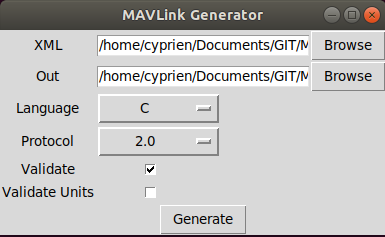
\includegraphics[scale=0.75]{img/mavgen.png}
    \caption{Générateur MAVGEN}
    \label{fig:mavgen}
\end{figure}
Le GUI permet de choisir le fichier source, le repertoire cible ainsi que le langage et la version de MAVLINK désirée. 
Une fois la génération terminée en langage C, on retrouve nos fichiers au sein de la librairie MAVLINK : 
\begin{figure}[ht]
	\centering
    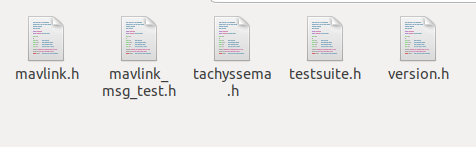
\includegraphics[scale=0.5]{img/fichiersC.png}
    \caption{Fichiers .C générés }
    \label{fig:mavgen}
\end{figure}
\subsubsection{Utilisation du message dans un projet}
A présent, il est possible de  transmettre le nouveau message via le protocole MAVLINK. On retrouve bien dans les fichiers générés la structure de notre message: 
\lstset{style=C_Style}
\begin{lstlisting}[caption={Structure personnalisée},captionpos=b, label={lst:custom_struct __mavlink_message_test_t}]
MAVPACKED(
	typedef struct __mavlink_custom_struct_t {
		uint32_t var1; /*<  Comment variable 1*/
		uint32_t var2; /*<  Comment variable 2*/
		uint32_t var3; /*<  Comment variable 3*/
		uint32_t var4; /*<  Comment variable 4*/
	}) mavlink_custom_struct_t;
\end{lstlisting}


\newpage
\section{Mise en œuvre du protocole MAVLINK pour le système OptSys}
\subsection{Utilisation des fonctions incluses dans le protocole MAVLINK}
\subsubsection{Heartbeat}
Il faudra utiliser l'échange Heartbeat précédemment décrit pour s'assurer que la caméra est bien connectée au réseau. Il reste cependant à définir à quelle période ce type de message doit être émit par la caméra pour la considérer connectée ou non au réseau.
\subsubsection{Informations et paramètres de la caméra}
Pour obtenir les informations de la caméra, l’échange « Camera informations » sera établit et permettra à la caméra de transmettre la structure de données « CAMERA
\_INFORMATIONS » renvoyant l’ensemble des paramètres présents sur la figure 2.

\

Les messages MAV\_CMD\_REQUEST\_CAMERA\_SETTINGS et MAV\_CMD\_SET
\_CAMERA\_MODE permettront d’obtenir et/ou modifier les paramètres suivants :
\begin{itemize}
	\item Le zoom de la caméra
	\item Le focus de la caméra
	\item Le mode dans lequel se trouve la caméra (prise d’image ou de vidéo)

\end{itemize}


\subsubsection{Lancement et arrêt d'une diffusion vidéo}

Pour activer la diffusion vidéo de la caméra, nous utiliserons la commande MAV
\_CMD\_VIDEO\_START\_STREAMING.
\newline 
\par
    Pour arrêter  la diffusion vidéo de la caméra, nous utiliserons la commande MAV
\_CMD\_VIDEO\_STOP\_STREAMING.

\subsection{Ajout de fonctions publiques au protocole MAVLINK}

La création d’un dialecte publique sera mis en œuvre pour ajouter des définitions de messages publiques non existants via le protocole MAVLINK qui seront utiles à la caméra.
Par exemple l'ajout de messages pour gérer la saturation et la teinte de la vidéo. 

\subsection{Ajout de fonctions privées au protocole MAVLINK}

Certains attributs de la caméra ne seront pas visibles par le client. Comme par exemple :  
\begin{itemize}
	\item L'offset
	\item La matrice
	\item Le seuil  
	\item La colorimétrie
	\item Le numéro de série etc ..

\end{itemize}
\

Pour se faire, un dialecte privé contentant la définition de ces messages sera établit. 
